\documentclass[border=6pt]{standalone}
\usepackage[T1]{fontenc}
\usepackage{lmodern}
\usepackage{amsmath,amssymb}
\usepackage{tikz}
\usetikzlibrary{arrows.meta,calc,positioning,shapes.misc,decorations.pathreplacing}
\definecolor{hyp}{RGB}{38,94,160}
\definecolor{half}{RGB}{204,110,20}
\definecolor{conj}{RGB}{176,32,40}
\definecolor{side}{RGB}{100,100,110}
\definecolor{planeA}{RGB}{232,240,250}
\definecolor{planeB}{RGB}{252,240,226}
\definecolor{planeC}{RGB}{250,232,232}

\definecolor{base}{RGB}{226,229,234}
\definecolor{fc}{RGB}{196,216,238}
\definecolor{q0}{RGB}{238,170,100}
\definecolor{qq}{RGB}{210,220,232}
\begin{document}
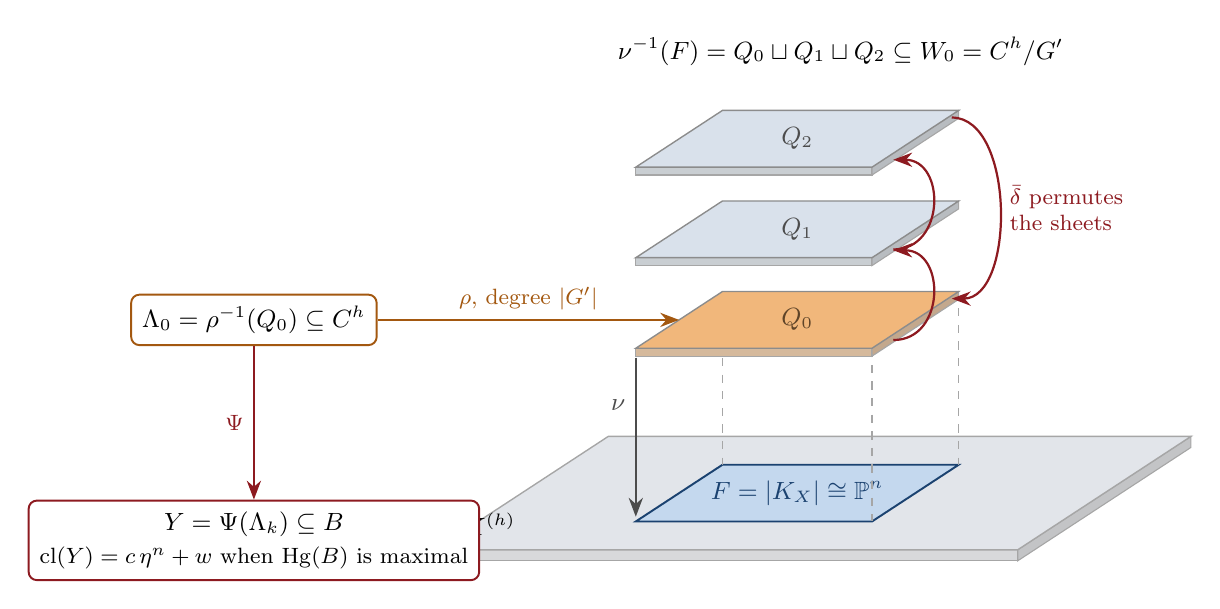
\begin{tikzpicture}[x={(1cm,0cm)}, y={(0.55cm,0.36cm)}, z={(0cm,1cm)},
  >={Stealth[length=2.4mm,width=1.8mm]}, font=\small]

% X^(h)
\filldraw[fill=base!70!black!40, draw=black!35, line width=0.4pt]
  (0,0,0) -- (7.4,0,0) -- (7.4,0,-0.14) -- (0,0,-0.14) -- cycle;
\filldraw[fill=base!60!black!50, draw=black!35, line width=0.4pt]
  (7.4,0,0) -- (7.4,4,0) -- (7.4,4,-0.14) -- (7.4,0,-0.14) -- cycle;
\filldraw[fill=base, draw=black!35, line width=0.5pt]
  (0,0,0) -- (7.4,0,0) -- (7.4,4,0) -- (0,4,0) -- cycle;
\node[anchor=south west, font=\small] at (0.15,0.15,0) {$X^{(h)}$};
% F = |K_X|
\filldraw[fill=fc, draw=hyp!70!black, line width=0.7pt]
  (2,1,0) -- (5,1,0) -- (5,3,0) -- (2,3,0) -- cycle;
\node[font=\small, text=hyp!70!black] at (3.5,2,0) {$F=|K_{X}|\cong\mathbb{P}^{n}$};

% guide lines from the lowest sheet to F
\draw[black!35, dashed, line width=0.4pt] (5,1,2.2) -- (5,1,0);
\draw[black!35, dashed, line width=0.4pt] (5,3,2.2) -- (5,3,0);
\draw[black!35, dashed, line width=0.4pt] (2,3,2.2) -- (2,3,0);

% the three sheets, bottom to top
\foreach \z/\c/\t/\tc in {2.2/q0/{Q_{0}}/q0!40!black, 3.35/qq/{Q_{1}}/black!70, 4.5/qq/{Q_{2}}/black!70}{
  \filldraw[fill=\c!75!black!55, draw=black!35, line width=0.4pt]
    (2,1,\z) -- (5,1,\z) -- (5,1,\z-0.1) -- (2,1,\z-0.1) -- cycle;
  \filldraw[fill=\c!65!black!60, draw=black!35, line width=0.4pt]
    (5,1,\z) -- (5,3,\z) -- (5,3,\z-0.1) -- (5,1,\z-0.1) -- cycle;
  \filldraw[fill=\c!85!white, draw=black!45, line width=0.5pt]
    (2,1,\z) -- (5,1,\z) -- (5,3,\z) -- (2,3,\z) -- cycle;
  \node[text=\tc, font=\small] at (3.5,2,\z) {$\t$};
}

% nu
\draw[->, line width=0.8pt, black!70] (2,1,2.08) -- node[left, pos=0.3] {$\nu$} (2,1,0.06);

% delta-bar
\draw[->, line width=0.8pt, conj!80!black] (5.05,1.4,2.16) to[out=0, in=0, looseness=1.5] (5.05,1.4,3.3);
\draw[->, line width=0.8pt, conj!80!black] (5.05,1.4,3.31) to[out=0, in=0, looseness=1.5] (5.05,1.4,4.45);
\draw[->, line width=0.8pt, conj!80!black] (5.05,2.75,4.5) to[out=0, in=0, looseness=0.9]
  node[right, pos=0.5, align=left, font=\footnotesize] {$\bar\delta$ permutes\\the sheets} (5.05,2.75,2.2);

% Lambda_0 and Y
\node[draw=half!80!black, fill=white, rounded corners=3pt, line width=0.7pt, inner sep=4pt]
  (Lam) at (-3.4,2,2.2) {$\Lambda_{0}=\rho^{-1}(Q_{0})\subseteq C^{h}$};
\node[draw=conj!80!black, fill=white, rounded corners=3pt, line width=0.7pt, inner sep=4pt, align=center]
  (Y) at (-3.4,2,-0.6) {$Y=\Psi(\Lambda_{k})\subseteq B$\\[1pt]
  {\footnotesize $\mathrm{cl}(Y)=c\,\eta^{n}+w$ when $\mathrm{Hg}(B)$ is maximal}};
\draw[->, line width=0.8pt, half!80!black] (Lam.east) -- node[above, font=\footnotesize] {$\rho$, degree $|G'|$} (2,2,2.2);
\draw[->, line width=0.8pt, conj!80!black] (Lam.south) -- node[left, font=\footnotesize] {$\Psi$} (Y.north);

\node[anchor=south, font=\small, align=center] at (3.5,3,4.95)
  {$\nu^{-1}(F)=Q_{0}\sqcup Q_{1}\sqcup Q_{2}\subseteq W_{0}=C^{h}/G'$};
\end{tikzpicture}
\end{document}
